\documentclass[11pt]{article}

% To produce a letter size output. Otherwise will be A4 size.
\usepackage[letterpaper]{geometry}
\usepackage{graphicx}

% For enumerated lists using letters: a. b. etc.
\usepackage{enumitem}

\topmargin -.5in
\textheight 9in
\oddsidemargin -.25in
\evensidemargin -.25in
\textwidth 7in

\begin{document}

% Edit the following putting your first and last names and your lab section.
\author{Atageldi Altyyev\\
CSE-30 (lab 06L)}

% Edit the following replacing X with the HW number.
\title{CSE 30: Midterm\\}

% If you put nothing today's date will be included. Alternatively, uncomment the next line and put the date you want to appear
\date{October 15, 2020}
\maketitle

% ========== Begin questions here

\textbf{Question 1: Getting random elements from arrays of different sizes.}
\\Getting any element from the array of any size at the given index always takes constant time (about ~0 ms).\\
Regardless of how big the array is, 'get' function will only address the memory location of the provided index. $f(n) = 0$.\\
Here is the most useful table ever:\\
\begin{displaymath}
\begin{array}{|c|c|}
\textit{Number of Elements} & \textit{Access Time (ms)}\\
\hline
 424321 & 0\\
 252174 & 0\\
 9992471 & 0\\
 4196 & 0\\
 21110342 & 0\\
\end{array}
\end{displaymath}

\textbf{Question 2: Getting a value at a given position from a linked list.}
\\For any value, other than the first and the last ones, the loop has to iterate the amount of times given by the position. The size of the linked list won't matter because the amount of iterations in 'get' function will only depend on the given position.
\\In the following table we will be reading from a \textbf{constant} position from lists of different sizes to show that the access time does not depend on the size.
\begin{displaymath}
\begin{array}{|c|c|}
\textit{Number of Elements} & \textit{Access Time (ms)}\\
\hline
 500001 & 2 \\
 4385080 & 2\\
 7892791 & 1\\
 6044371 & 1\\
 79218739 & 1\\
 70799205 & 2\\
\end{array}
\end{displaymath}
\\ $f(n) = c$, where $c$ is the given position (in example above $c=500000$). In other words, there is no dependency on the size of the list.\\
\\In contrast, in the following chart we will be reading from a \textbf{random} position, to show that access time depends on the position number proportionally ($f(c) = c$).\\
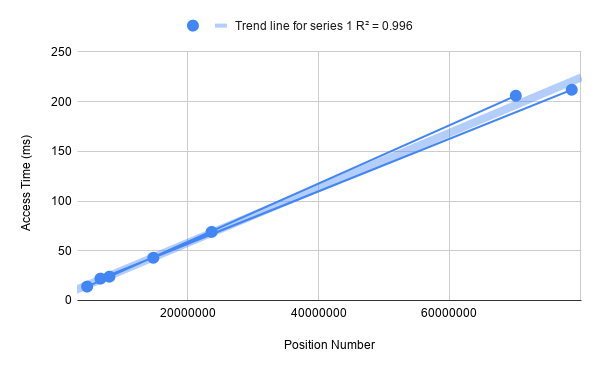
\includegraphics[width=\textwidth]{chart1.png}
\\Concluding, the relationship between the size and the access time is $f(n) = c$ meaning that there is no dependency on the size of the list.
\\
\\
\textbf{Question 3: Insertion at the end of the array.}
\\When inserting an element at the end of the array, it is equivalent to appending an element. Meaning, there are no repeated operations to perform. The function just inserts the number into the last position (counter). Therefore, it is not dependent on the size of the array because it doesn't have to shift anything or change the values of other elements.
\\$f(n) = 0$.

\begin{displaymath}
\begin{array}{|c|c|}
\textit{Number of Elements} & \textit{Insertion Time (ms)}\\
\hline
 992696996 & 0\\
 46894401 & 0\\
 205009095 & 0\\
 179150774 & 0\\
\end{array}
\end{displaymath}

\newpage
\textbf{Question 4: Insertion at the beginning of the array.}
\\When inserting at beginning of the array, what's happening is that all elements of the array will be shifted to the right by index 1. The amount of iterations is straightly dependent on the size of the array. Furthermore, it is equal to the size of the array. The dependency is $f(n) = n$.
\\The following chart proves the dependency.

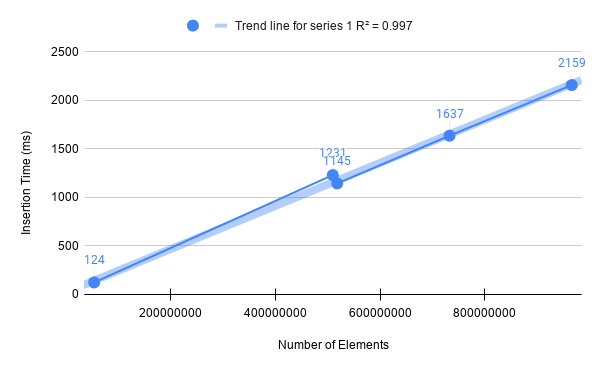
\includegraphics[width=\textwidth]{chart.png}

\newpage
\textbf{Question 5: Insertion at the end of the linked list.}
\\Insertion at the end of the list is an 'append' function. It will have constant execution time, regardless of the size of the list. All it does is taking the last Node and making it's 'next' point to a newly created Node.
\\$f(n) = 0$. The following table shows that.

\begin{displaymath}
\begin{array}{|c|c|}
\textit{Number of Elements} & \textit{Insertion Time (ms)}\\
\hline
 393559 & 0\\
 72741810 & 0\\
 3279602 & 0\\
 1420676 & 0\\
\end{array}
\end{displaymath}

\textbf{Question 6: Insertion in the beginning of the linked list.}
\\Insertion in the beginning of the linked list is a 'prepend' function. It will also have a constant execution time and all it does is creating a Node with 'next' pointing to 'head', and making 'head' point to a new node.
\\$f(n) = 0$. The following table shows that.

\begin{displaymath}
\begin{array}{|c|c|}
\textit{Number of Elements} & \textit{Insertion Time (ms)}\\
\hline
 9309873 & 0\\
 5161950 & 0\\
 446 & 0\\
 59744808 & 0\\
\end{array}
\end{displaymath}

\end{document}
